\input{doctools/latex/magazine_template.tex}   %Page setup
\input{doctools/latex/mycommands.tex}       %Some useful commands

% Figure search path
\graphicspath{
              {figs/} % Figures drawn with xfig
              {pngs/} % Other graphics files
}

\begin{document}





%%%%%%%%%%%%%%%%%%%%%%%%%%%%%%%%%%%%%%%%%%%%%%%%%%%%%%%%%%%%%%%%%%%%
%Title
%%%%%%%%%%%%%%%%%%%%%%%%%%%%%%%%%%%%%%%%%%%%%%%%%%%%%%%%%%%%%%%%%%%%
\begin{center}
	{\huge ASCII command interface for the AVR Butterfly}\\
	\today
\end{center}

%%%%%%%%%%%%%%%%%%%%%%%%%%%%%%%%%%%%%%%%%%%%%%%%%%%%%%%%%%%%%%%%%%%%
%Table of contents
%%%%%%%%%%%%%%%%%%%%%%%%%%%%%%%%%%%%%%%%%%%%%%%%%%%%%%%%%%%%%%%%%%%%
\tableofcontents


\section{Making connections to the Butterfly}

\begin{figure}[ht]
    \begin{center}
        \includegraphics[clip,scale=1]{usart_pinout}
        \caption{Connections needed for the AVR Butterfly.\label{fig:connections}}
    \end{center}
\end{figure}



\section{The debug output}

% See the termgrab.sh script for details about creating grab.eps
\begin{figure}[ht]
    \begin{center}
        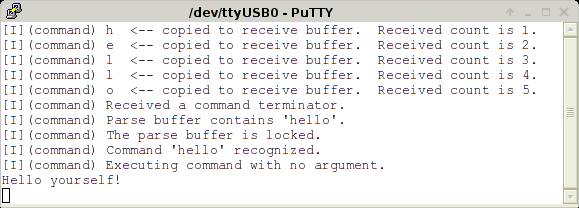
\includegraphics[clip,scale=0.5]{grab.eps}
        \caption{Terminal output showing debug information.\label{fig:termgrab}}
    \end{center}
\end{figure}

\section{The command list}

\lstset{language=C}
\begin{lstlisting}[float,frame=single]
/* An array of command_structs will contain our remote commands */
struct command_struct command_array[] ={
    // The junk function
    {"junk", // Name
    "hex", // Argument type
    2, // Maximum number of characters in argument
    &junkfunc,
    "Some junk"},
    // The crap function
    {"crap",
    "none",
    0,
    &crapfunc,
    "Some crap"},
    // End of table indicator.  Must be last.
    {"","",0,0,""}
};
\end{lstlisting}




\bibliography{latex/ecrefs}
\end{document}
